\documentclass[preview]{standalone}

\usepackage{amsmath}
\usepackage{amssymb}
\usepackage{stellar}
\usepackage{definitions}
\usepackage{tikz}

\begin{document}

\id{manifolds-definitions}
\genpage

\section{Definitions}

\begin{snippetdefinition}{manifold-definition}{Manifold}
    An \textit{\(n\)-manifold} is a \topologicalspace \(T\) where
    every point TODO... % https://en.wikipedia.org/wiki/Manifold#Mathematical_definition
\end{snippetdefinition}

\begin{snippet}{manifold-definition-illustration}
    \begin{center}
        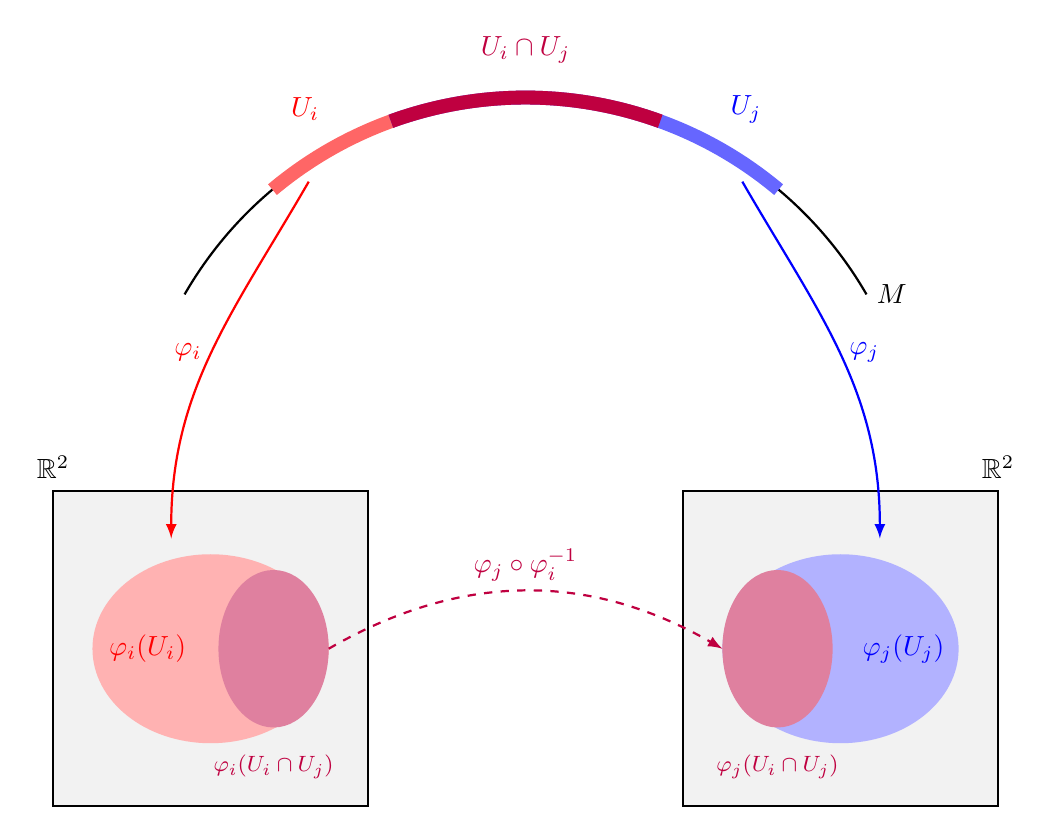
\begin{tikzpicture}
            \draw[thick] (150:5) arc (150:30:5) node[right] {$M$};
            \draw[line width=5pt, red!60] (130:5) arc (130:70:5);
            \draw[line width=5pt, blue!60] (110:5) arc (110:50:5);
            \draw[line width=5pt, purple] (110:5) arc (110:70:5);
            \node[red] at (120:5.6) {$U_i$};
            \node[blue] at (60:5.6) {$U_j$};
            \node[purple] at (90:5.6) {$U_i \cap U_j$};
            \filldraw[fill=gray!10, draw=black, thick] (-6,-4) rectangle (-2,0);
            \node at (-6, 0.3) {$\mathbb{R}^2$};
            \filldraw[fill=gray!10, draw=black, thick] (2,-4) rectangle (6,0);
            \node at (6, 0.3) {$\mathbb{R}^2$};
            \fill[red!30] (-4,-2) ellipse (1.5 and 1.2);
            \fill[purple!50] (-3.2,-2) ellipse (0.7 and 1);
            \node[red] at (-4.8,-2) {$\varphi_i(U_i)$};
            \node[purple, font=\footnotesize] at (-3.2,-3.5) {$\varphi_i(U_i \cap U_j)$};
            \fill[blue!30] (4,-2) ellipse (1.5 and 1.2);
            \fill[purple!50] (3.2,-2) ellipse (0.7 and 1);
            \node[blue] at (4.8,-2) {$\varphi_j(U_j)$};
            \node[purple, font=\footnotesize] at (3.2,-3.5) {$\varphi_j(U_i \cap U_j)$};
            \draw[-latex, red, thick] (125:4.8) to[out=240, in=90] node[left] {$\varphi_i$} (-4.5, -0.6);
            \draw[-latex, blue, thick] (55:4.8) to[out=300, in=90] node[right] {$\varphi_j$} (4.5, -0.6);
            \draw[-latex, purple, thick, dashed] (-2.5, -2) to[out=30, in=150] node[above] {$\varphi_j \circ \varphi_i^{-1}$} (2.5, -2);
        \end{tikzpicture}
    \end{center}
\end{snippet}

\end{document}